\chapter{UNIXシェル}
ここでは簡易版のUNIXシェル(以下では myshell\footnote{
ソースコードは
\url{https://github.com/tctsigemura/SystemPrograming}からダウンロードできる.
}と呼ぶ)を紹介する.
これの内容を理解し,更に,改造したりすることで,
これまでに学習した様々なシステムコール等の意味を深く理解する.

\section{UNIXのシェルとは}
UNIXのシェルはCLI(Command Line Interface)方式の
コマンド行インタプリタ\footnote{
macOSのFinderや,WindowsのExplorerはGUI版のシェルである.}である.
ユーザが入力したコマンド行を解析し実行するインタプリタの一種である.

macOSでも\|sh|,\|bash|,\|ksh|,\|zsh|,\|csh|,\|tcsh|等,
多種類のUNIXのシェルが利用可能である.
macOSの場合,標準のログインシェル\footnote{
ターミナルを開いたとき最初に使用されるシェルのこと.
}は\|bash|になっているが,好みで変更する\footnote{
chshコマンドで変更する.}ことも可能である.
これらのUNIXシェルはどれも高機能なものであり,
かなり大きなプログラムである.
UNIXシェルは最低でも次の機能を持っている.

\begin{enumerate}
\item 外部コマンド(プログラム)を起動する機能
\item カレントディレクトリを変更する機能
\item 環境変数などの変数管理機能
\item 入出力のリダイレクト機能やパイプ機能(\|<|,\|>|,\|>>|,\verb;|;)
\item ジョブ管理機能(jobs,fg,bgなど)
\item ファイル名の展開機能(ワイルドカード)
\item 繰り返しや条件判断機能
\item スクリプトの実行機能
\end{enumerate}

\section{簡易UNIXシェル(myshell)}
myshellはC言語で70行以内で記述可能な簡易版UNIXシェルである.
コマンド行は空白区切りの文字列とする.
myshellは以下の二つの機能しか持たない.

\begin{enumerate}
\item 外部コマンド(プログラム)を起動する機能
\item カレントディレクトリを変更する機能
\end{enumerate}

本章はmyshellの構造を学び,
「環境変数の管理機能」,
「入出力のリダイレクト機能」等を
myshellに追加できるようになることを目標とする.

\subsection{基本構造(\texttt{main()}関数)}
myshell は,コマンド行の「入力」,「解析」,「実行」を
入力がEOFになるまで繰り返す.
これを,リスト\ref{myshellMain}の\|main()|関数で行う.
\|main()|関数の動作は次の通りである.

\lstinputlisting[label=myshellMain
  ,caption=メインループ
  ,float=btp, numbers=left]{Lst/myshellMain.c}

\begin{enumerate}
\item 6行で
  \|fgets()|関数\footnote{
    \texttt{fgets()}関数はC言語の標準ライブラリ関数である.
  }を用いてコマンド行を\|buf|配列に入力する.
  \|buf|配列には\|'\n'|,\|'\0'|で終端された文字列が格納されるはずである.
\item 10行では,
  \|strchr()|関数\footnote{
    \texttt{strchr()}関数はC言語の標準ライブラリ関数である.
  }を用いてバッファに\|'\n'|が格納されていることを確認する.
  格納されていない場合は,
  「コマンド行が長すぎてバッファに入り切らない」エラーが発生した場合である.
  簡易版のシェルなのでエラーから復旧は諦めて,
  エラーメッセージを表示してシェルを終了する.
\item 14行では,
  後で説明する\|parse()|関数を用いて\|buf|配列のコマンド行を解析し,
  execveシステムコールに渡す\|args|配列を作る.
  もしも,コマンド行の文字列が多すぎて配列に格納しきれない時は,
  \|parese()|関数が\|0|を返すのでエラーメッセージを表示して入力を無視する.
\item 18行では,
  \|args|配列にコマンドが格納されていることを確認した後,
  後で説明する\|execute()|関数に依頼して\|args|配列のコマンドを実行する.
\end{enumerate}

\subsection{コマンド行の解析(\texttt{parse()}関数)}
\|parse()|関数がコマンド行を解析し\|execve()|システムコールの
第2引数で使用できる\|argv|形式に変換する.
リスト\ref{myshellParse}にmyshellの\|parse()|関数を示す.
動作は次の通りである.

\lstinputlisting[label=myshellParse
  ,caption=コマンド行の解析ルーチン
  ,float=btp, numbers=left]{Lst/myshellParse.c}

\begin{enumerate}
\item コマンド行に入力された文字列と,
  解析結果を格納する文字列配列を引数に呼出される.
\item 4行では,
  \|isspace()|関数\footnote{
    \texttt{isspace()}関数は空白文字を判定するC言語の標準ライブラリ関数である.
    スペース,タブ,改行などを空白と判定する.
  }を用いて文字列に先行する空白を読み飛ばす(ポインタ\|p|を進める).
  その際,5行で空白を文字列の終端記号である\|'\0'|に置き換えておく.
\item 6行では,解析処理の完了を判断する.
  空白を読み飛ばした後で最初に見つかった文字が\|'\0'|なら,
  コマンド行の最後まで達しているので\|for(;;)|ループを脱出し解析を終了する.
  または,\|args|配列のサイズを超えそうになっていた場合は,
  文字列が多すぎてこれ以上処理できないので終了する.
\item 処理が7行に進むのは,
  新しく次の文字列が見つかった場合である.
  新しい文字列の開始位置(ポインタ)を\|args|配列に記録する.
\item 8行では,\|isspace()|関数を用いて文字列を終端する空白を探す.
  終端が見つかったら\|for(;;)|ループの先頭に戻り,
  4,5行で空白を\|'\0'|に書換えC言語の文字列として完成する.
\item 11,12行では,
  文字列配列に配列の終端を表す\|NULL|を書込み\|parse()|関数を終了する.
  その際,コマンド行の最後まで解析が終わっていれば\|1|(true)を,
  そうでなければ\|0|(false)を返す.
\end{enumerate}

\begin{myfig}{btp}{\texttt{parse()}関数の実行結果例}{myshellArgs}
  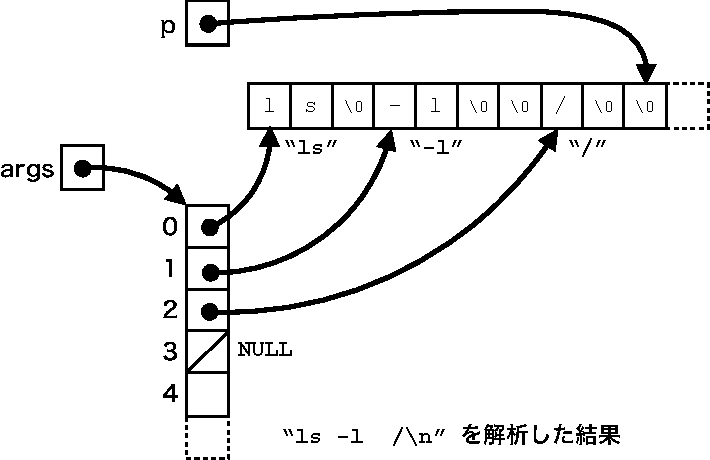
\includegraphics[scale=0.8]{Fig/myshellArgs-crop.pdf}
\end{myfig}

\figref{myshellArgs}に\|parse()|関数実行後のデータ構造の例を示す.
この例は,コマンド行文字列
~\texttt{"ls{\textvisiblespace}-l{\textvisiblespace}{\textvisiblespace}/{\bs}n"}~
を解析した後のデータ構造である.
渡した1つの文字列の空白を\|'\0'|で上書きし
\|"ls"|,\|"-l"|,\|"/"|の3つの文字列が作られている\footnote{
  リスト\ref{myshellParse}の5行で\texttt{'{\bs}0'}に書換えている.}.
文字列配列の終端は\|NULL|で表現する.
\|args|配列は各文字列の先頭を指すポインタを格納する\footnote{
  リスト\ref{myshellParse}の7行でポインタを\texttt{args}配列に格納している.
}ことで文字列配列を表現する.
文字列の最後の \|'\n'| は \|'\0'| に書き換わっている\footnote{
  \texttt{'{\bs}n'}は\texttt{isspace()}関数により空白と判断される.
}.

\subsection{コマンドの実行(\texttt{execute()})}
リスト\ref{myshellExecute}にmyshellの\|execute()|関数を示す.
この関数は\|parse()|関数が作った\|args|配列を受け取り,
内部コマンドなら自分で実行し,
外部コマンドなら子プロセスを作って実行させる.


\lstinputlisting[label=myshellExecute
  ,caption=コマンドの実行ルーチン
  ,float=btp, numbers=left]{Lst/myshellExecute.c}

2行ではコマンドの名前を調べている.
cd コマンドは内部コマンドなので,
5行で自ら\|chdir()|システムコールを実行している\footnote{
  内部コマンドを追加するときは,cd コマンドと同様に,ここに追加する.}.
7行以下は外部コマンドの処理である.
9行で子プロセスを作り,14行で子プロセスがコマンドを実行する.
親プロセスは18行で子プロセスの終了を待つ.

\section*{課題 No.11}

\begin{enumerate}
\item myshell に環境変数を追加するコマンド setenv ,
  削除するコマンド unsetenv を追加しなさい.
\item myshell にリダイレクト機能を追加しなさい.
\end{enumerate}
